%!TEX root = ../template.tex
%%%%%%%%%%%%%%%%%%%%%%%%%%%%%%%%%%%%%%%%%%%%%%%%%%%%%%%%%%%%%%%%%%%%
%% chapter3.tex
%% NOVA thesis document file
%%
%% Chapter with a short latex tutorial and examples
%%%%%%%%%%%%%%%%%%%%%%%%%%%%%%%%%%%%%%%%%%%%%%%%%%%%%%%%%%%%%%%%%%%%

\typeout{NT FILE chapter3.tex}%


\chapter{Results}
\label{cha:results}

The algorithms seen in \ref{sec:Proposed_Decision_Algorithms}, namely, \label{subsec:decision_algorithms} \glsxtrshort{A-JO}, \glsxtrshort{A-CLF-S} and \glsxtrshort{A-CLF-I},  are going to be implemented in different systems, in a unicycle~\ref{subsec:unicycle_simul_setup} and orbital system~\ref{subsec:orbital_simul_setup}, and subject to different types of experiments according to the system in question (unicycle~\ref{subsubsec:unicyle_type_of_experiments} or orbital~\ref{subsubsec:orbital_type_of_experiments}). In each of the contexts, there is an analisys of the techniques and a comparation between them highlingting some relevant data.

\section{Setup}
\label{sec:setup}

\subsection{Decision Algorithms}
\label{subsec:decision_algorithms}

%The respective algorithms have some parameters to be defined to attend the problem needs.

\subsubsection{\glsxtrshort{A-JO}}
\label{subsubsec:A-JO_parameters}

The parameter \(\alpha\) is optimized based on a cost function \(g_{\xVec_0}(\alpha)\)~\ref{eq:Cost_Function_Alpha}, which takes \(N=6000\) samples and has the weight cost matrices \(\mathbf{Q} = \mathbf{I}_{2\times 2} \) and \(\mathbf{R} = 5 \hspace{0.1em}^.\mathbf{I}_{2\times 2} \).\\

The function \(SPS\)~\ref{eq:CLF-CBF_RK4_Propagation} and \(DGF\)~\ref{eq:discrete_gradient_function} parameters used in these experiments are given by:


 \bgroup
 \rowcolors{1}{}{GhostWhite}
 \begin{xltabular}{\textwidth}{ccccc}
   \caption{SPS~\ref{eq:CLF-CBF_RK4_Propagation} Parameters}
   \label{tab:A-JO:SPS_parameters}\\
   \toprule
   \rowcolor{Gainsboro}
   $f$ &  $\xVec_0$ & $N$ & $\Delta t$  & $V, \hspace{0.25em} h, \hspace{0.25em} \alpha_{ini}$  \\
   \midrule
     \ref{eq:unicycle_model} or \ref{}          &  \ref{subsubsec:unicyle_type_of_experiments} or \ref{subsubsec:orbital_type_of_experiments}       & 6000          & 0.005  &   \ref{subsubsec:Unicyle_CLF-CBF_Experiment_Setup} or \ref{}\\
   \midrule
   \end{xltabular}
 \egroup




  \bgroup
 \rowcolors{1}{}{GhostWhite}
 \begin{xltabular}{\textwidth}{ccccc}
   \caption{DGF~\ref{eq:discrete_gradient_function} Parameters}
   \label{tab:A-JO:DGF_parameters}\\
   \toprule
   \rowcolor{Gainsboro}%
   $nS$ &  $devS$ & $dev$ & $g_{\xVec_0}(\alpha)$  & $\alpha_{ini}$  \\
   \midrule
     3          &  0.01        & 0.005        &  \ref{eq:Cost_Function_Alpha}   &   \ref{subsubsec:Unicyle_CLF-CBF_Experiment_Setup} or \ref{}\\
   \midrule
   \end{xltabular}
 \egroup


\newpage %so para ajeitar

 \subsubsection{Double \glsxtrshort{CLF}}
\label{subsubsec:double_CLF_parameters}

The double \glsxtrshort{CLF} algorithms~\ref{subsec:Double_CLF} functions parameters are defined by:

 \bgroup
 \rowcolors{1}{}{GhostWhite}
 \begin{xltabular}{\textwidth}{ccccc}
   \caption{NCDV~\ref{eq:New_Equlibrium_Point_DirVec_CLF-CBF_RK4} Parameters}
   \label{tab:Double-CLF:NCDV_parameters}\\
   \toprule
   \rowcolor{Gainsboro}%
   $f$ &  $\xVec_0$ & $N$ & $\Delta t$  & $V, \hspace{0.25em} h$  \\
   \midrule
     \ref{eq:unicycle_model} or \ref{}   &  \ref{subsubsec:unicyle_type_of_experiments} or \ref{subsubsec:orbital_type_of_experiments}        & 6000          & 0.005  &   \ref{subsubsec:Unicyle_CLF-CBF_Experiment_Setup} or \ref{}\\
   \midrule
   \end{xltabular}
 \egroup


  \bgroup
 \rowcolors{1}{}{GhostWhite}
 \begin{xltabular}{\textwidth}{lcccc}
   \caption{Double \glsxtrshort{CLF}~\ref{subsec:Double_CLF} Transition Parameters}
   \label{tab:Double-CLF:NCDV_parameters}\\
   \toprule
   \rowcolor{Gainsboro}%
   Algorithms   & $\zeta$  & $\mu$  & $tol$   & $tol_2$            \\
   \midrule
    \glsxtrshort{A-CLF-S}~\ref{subsubsec:CLFs_Summed_Algorithm}        & 1         & $\frac{V_N(\xVec)}{V_C(\xVec)}$        & $0.03^.V_C(\xVec_0)$         & 999          \\
    \glsxtrshort{A-CLF-I}~\ref{subsubsec:CLFs_Independent_Algorithm}   & ---       & ---                                    & $0.05^.V_C(\xVec_0)$         & 50        \\
    \midrule
   \end{xltabular}
 \egroup

With \(V_C(\xVec)\) and \(V_N(\xVec)\) following the same formulation but different equilibrium points.

\subsection{Unicycle}
\label{subsec:unicycle_simul_setup}

This example consists in drive a unicycle to a specific location \(\mathbf{ref} \in \mathbb{R}^2\). Drive a vehicle implies the possibilitie of founding some obstacles, and while a collision could mean a fatality there are other factors as the fuel/energy consumed and how fast to achieve the wanted location, that beeing said, this represents an example of safety-critical control subject to an optimization of its path. \par

\subsubsection{Dynamics}
\label{subsec:unicycle_dynamics}

This unicycle doesn't loose traction in its wheels, and it is not constrained by its control inputs or its consume. It is also not affected by any perturbation such as drag force characteristic from the enviroment. It can be modeled mathematically as a relative two degree system:

\begin{equation}
    \begin{bmatrix} \dot{x} \\ \dot{y} \\ \dot{\theta} \end{bmatrix} = \begin{bmatrix} \frac{1}{2}cos \theta & \frac{1}{2}cos \theta \\  \frac{1}{2}sin \theta & \frac{1}{2}sin \theta \\ -L & L  \end{bmatrix} \begin{bmatrix} v_l \\ v_r\end{bmatrix}
    \label{eq:unicycle_model}
\end{equation}


Where the states are the \((x,y)\) 2D position and \(\theta\) the orientation, and the control inputs \(\uVec \in \mathbb{R}^2\) are the left and right wheel speed \(v_l\) and \(v_r\) respectively, in addition, the constant \(L = 10 m^{-1}\) refers to the inverse of the distance between the two wheels. 

\subsubsection{\glsxtrshort{CLF-CBF} Formulation}
\label{subsubsec:Unicyle_CLF-CBF_Experiment_Setup}

As the decision algoritms subject to comparations~\ref{subsec:decision_algorithms} are governed by the \glsxtrshort{CLF-CBF}~\ref{sec:clf_cbf} backstepping technique~\ref{sub:backstepping}, the system can be written as:


\begin{equation}
    \begin{array}{l}
        \dot{\xVec} = f_0(\xVec) +  g_0(\xVec, \xi)\uVec \\
        \dot{\xi} = f_1(\xVec, \xi) + g_1(\xVec, \xi)\uVec
    \end{array}
    \label{eq:second_order_unicycle_model_backstepp}
\end{equation}

With \(\xVec =  \bigl[\begin{smallmatrix} x \\ y \end{smallmatrix}\bigr]\), \(\xi =  \bigl[\begin{smallmatrix} cos\theta \\ sin\theta \end{smallmatrix}\bigr]\), \(f_0(\xVec) = \mathbf{0}_{2 \times 1}\), \(g_0(\xVec, \xi) = \bigl[\begin{smallmatrix} \frac{1}{2}\xi_1 & \frac{1}{2}\xi_1 \\ \frac{1}{2}\xi_2 & \frac{1}{2}\xi_2 \end{smallmatrix}\bigr] \), \(f_1(\xVec, \xi) = \mathbf{0}_{2 \times 1}\) and \(g_1(\xVec, \xi) =  \bigl[\begin{smallmatrix} \xi_2L & -\xi_2^L \\ -\xi_1L &  \xi_2L \end{smallmatrix}\bigr]\). \par

Since it's a second-order system, to use backstepping and obtain the first-order solution \(\mathbf{k}_0(\xVec)\) it is considered the system:

\begin{equation}
    \dot{\xVec} = k_0(\xVec) 
    \label{eq:first_order_unicycle_model_backstepp}
\end{equation}

In order to make the vehicle to the wanted position is formulated a \glsxtrshort{CLF} \(V_0\) which actively works to stabilize the system in the constant \(\mathbf{ref}\).

\begin{subequations}
   \begin{align}
    &V_0(\xVec) = \frac{1}{2}(\xVec-\mathbf{ref})^{\top}(\xVec-\mathbf{ref}) \label{eq:V0_unicycle} \\
    &\dot{V_0}(\xVec) = \underbrace{(\xVec-\mathbf{ref})^{\top}}_{L_GV_0(\xVec)}\mathbf{k}_0(\xVec)  \label{eq:dot_V0_unicycle} \\
    &\gamma_0(\xVec)  = V_0(\xVec) \label{eq:CLF_gamma0_unicycle}
\end{align}
\label{eq:CLF0_unicycle}
\end{subequations}


The safety is defined according to the \glsxtrshort{CBF} \(h_0\) which restricts the obstacles using a ellipsoidal fit~\ref{eq:Ellipsoidal_fit}:

\begin{subequations}
   \begin{align}
    &h_0(\xVec) = (\xVec-\mathbf{p})^{\top}\mathbf{A_{xis}}(\xVec-\mathbf{p}) - 1 \label{eq:h0_unicycle} \\
    &\dot{h_0}(\xVec) = (\underbrace{(\mathbf{A_{xis}}(\xVec-\mathbf{p}))^{\top} + (\xVec-\mathbf{p})^{\top}\mathbf{A_{xis}}}_{L_Gh_0(\xVec)})\mathbf{k}_0(\xVec)  \label{eq:dot_h0_unicycle} \\
    &\alpha_0(\xVec, \alpha)  = \alpha h_0(\xVec) \label{eq:CBF_alpha0_unicycle}
\end{align}
\label{eq:CBF0_unicycle}
\end{subequations}


With \(\mathbf{A_{xis}} \in \mathbb{R}^{2 \times 2}_{\succeq 0}\) referent to the ellipse axis and \(\mathbf{p} \in \mathbb{R}^2\) equal to the center of the ellipse, both stipulated in \ref{subsubsec:unicyle_type_of_experiments}. Given the system \ref{eq:second_order_unicycle_model_backstepp}, the solution \(\mathbf{k}_0(\xVec)\), the \glsxtrshort{CLF} \(V\) and \glsxtrshort{CBF} \(V\) are defined (according to \ref{eq:Backstepp_CF}) as:


\begin{subequations}
   \begin{align}
    &V(\xVec, \xi) = V_0(\xVec) + 1 - cos(\theta - \theta_0(\xVec)) \label{eq:V_unicycle} \\
    &\dot{V}(\xVec, \xi) = \Bigl(\underbrace{((\xVec-\mathbf{ref}))^{\top}g_0(\xVec, \mathbf{k}_{0,\xi}) + sin(\theta -\theta_0(\xVec))\begin{bmatrix} -L & L \end{bmatrix}}_{L_GV(\xVec, \xi)} \Bigr) \mathbf{k}(\xVec)  \label{eq:dot_V_unicycle} \\
    &\gamma(\xVec)  = V(\xVec) \label{eq:CLF_gamma_unicycle}
\end{align}
\label{eq:CLF_unicycle}
\end{subequations}

\begin{subequations}
   \begin{align}
    &h(\xVec, \xi) = h_0(\xVec) - 1 + cos(\theta - \theta_0(\xVec)) \label{eq:h_unicycle} \\
    &\dot{h}(\xVec, \xi) = \Bigl(\underbrace{\bigl((\mathbf{A_{xis}}(\xVec-\mathbf{p}))^{\top} + (\xVec-\mathbf{p})^{\top}\mathbf{A_{xis}}\bigr)g_0(\xVec, \mathbf{k}_{0,\xi}) - sin(\theta -\theta_0(\xVec))\begin{bmatrix} -L & L \end{bmatrix}}_{L_Gh(\xVec, \xi)} \Bigr) \mathbf{k}(\xVec)  \label{eq:dot_h_unicycle} \\
    &\alpha(\xVec, \xi, \alpha = 1.2)  = \alpha h(\xVec, \xi) \label{eq:CBF_alpha_unicycle}
\end{align}
\label{eq:CBF_unicycle}
\end{subequations}


With \(\mathbf{k}_{0,\xi}(\xVec)\) and \(\theta(\xVec)\) given by:

\begin{align}
    &\mathbf{k}_{0,\xi}(\xVec) = \frac{\mathbf{k}_0(\xVec) }{|| \mathbf{k}_0(\xVec) ||}      \\
    &\theta_0(\xVec) = angle(\mathbf{k}_{0,\xi,1}(\xVec) + \mathbf{i} \hspace{0.2em} \mathbf{k}_{0,\xi,2}(\xVec))
\end{align}


\subsubsection{Type of Experiments}
\label{subsubsec:unicyle_type_of_experiments}

Falar do tipo de simulaçoes que se vai fazer que basicamente se resume a:\\
-falar dos valores tomados pelas axis das elipses\\
-falar do centro da elipse\\
-referir com base nos valores tomados pelas axis se é um circululo uma ellipse na horizontal, vertical ou diagonal relativamente ao uniciclo\\
-o valor inicial, posição e orientação dos sistema\\

NOTA: A medida que for escolhendo as simulaçoes ir metendo aqui a descrição delas (breve diria eu e direta).\par
Cada um dos experimentos descritos tem uma label ou nao mas seja como for sao destinguidos por ex:\textcolor{blue}{\underline{U.C.H.F.Pe)}} (Unicycle Circle Horizontal Far Perpendicular) talvez com cor diferente, tipo de letra, a bold ou sublinhadodo e com label mas não subsubsecção para não dar demasiado destque diria eu e confundir


Os experimentos que não entrarem aqui seram colocados nos anexos



\subsection{Orbital}
\label{subsec:orbital_simul_setup}

\subsubsection{Dynamics}
\label{subsubsec:orbital_dynamics}



\subsubsection{\glsxtrshort{CLF-CBF} Formulation}
\label{subsubsec:Orbital_CLF-CBF_Experiment_Setup}


\subsubsection{Type of Experiments}
\label{subsubsec:orbital_type_of_experiments}



\subsection{Some Data}
\label{subsec:some_data}

The techniques will be evaluated having in account a cost, given by the function \(g(\mathbf{X}, \mathbf{U})\), equivalent to \(g_{\bar{\xVec_0}}(\alpha)\) defined before~\ref{subsubsec:A-JO_parameters}, such as the weight cost matrices, \(\mathbf{Q} = \mathbf{I}_{2\times 2} \) and \(\mathbf{R} = 5 \hspace{0.1em}^.\mathbf{I}_{2\times 2} \), besides that the function is calculated with \(N=6000\) samples. It is also presented the time the system \(f\) takes to reach the equilibrium point.\par
The computational time for each experiment is given based on a single test (one sample Monte Carlo) using the the processor \emph{Intel(R) Core(TM) i7-8650U CPU @ 1.90GHz}.





\section{Experiments}
\label{sec:experiments}

The dynamical system propagation with respective decision algorithm~\ref{subsec:decision_algorithms} during the experiments is simulated using the \glsxtrlong{DP} integrative method~\ref{eq:Dormand-Prince_Tableu}. So, given a dynamical system (unicycle~\ref{eq:unicycle_model} or orbital~\ref{subsubsec:orbital_model}) \(f:\mathbb{R}^n \to \mathbb{R}^n\), at \( \xVec_0 \in \mathbb{R}^n\), a \glsxtrshort{CLF} \(V\) and a \glsxtrshort{CBF} \(h\), a sampling time \(\Delta t = 0.005\) seconds and a total of \(6000\) iterations totaling a simulation of \(30\) seconds:


\begin{equation}
    \begin{bmatrix} \mathbf{X} & \mathbf{U} \end{bmatrix} = SPS(f, \xVec_0, 6000, 0.005, V, h)\begin{bmatrix*}[l]conditions^* \gets V(\xVec) \geq tol \\ decision^* \gets \text{algorithms~\ref{subsec:decision_algorithms}} \\ integration^* \gets \text{\glsxtrshort{DP}~\ref{eq:Dormand-Prince_Tableu}}\end{bmatrix*}
    \label{eq:SPS_Experiments}
\end{equation}

Where \(SPS\) (State Propagation Simulation) is the algorithm~\ref{alg:State_Propagation_Simulation}.\\



\subsection{Unicycle}
\label{subsec:unicycle_experiments}

\underline{UCCL}
\label{ssssec:UCCL} %Unicycle Circular Close Looking


\begin{figure}[htbp]
  \begin{subfigure}{0.6\textwidth}
    \centering
    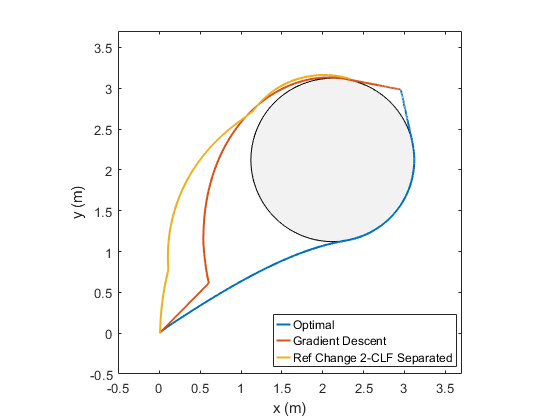
\includegraphics[width=0.99\linewidth]{UCCL.png}
  %\caption{A figure with two sub-figures!}
  \label{fig:UCCL_CostEvol}
  \end{subfigure}
  \begin{subfigure}{0.59\textwidth}
    \centering
    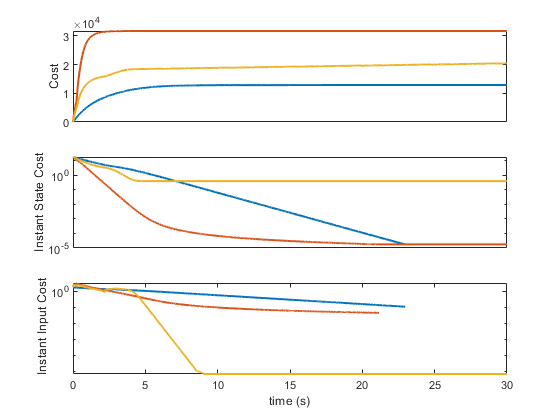
\includegraphics[width=0.95\linewidth]{UCCL_costs.png}
  %\caption{A figure with two sub-figures!}
  \label{fig:UCCL_trajectory}
  \end{subfigure}
  \caption{UCCL~\ref{}}
\label{fig:UCCLTrajectory_and_CostEvol}
\end{figure}


Although \glsxtrshort{A-JO} \(\alpha\) parameter is optimized its decision keeps beeing purely based on a \glsxtrshort{CLF-CBF} technique which lacks a bigger prediction horizon and thus taking the unicycle close to the obstacle as it is the way that approximates more to the \(\mathbf{ref}\) in the moment (less state cost compared to A-CLF-summed), obligating eventually to higher input values (generally bigger than CLF-summed) to deviate from the barrier safely while forcing as much as possible a speed of convergence to \(\mathbf{ref}\).  The \glsxtrshort{A-CLF-S} following the other point first results in a initially not so fast approximation to \txtref but (this forcing but informative point predicts an) to a shorter countour path and that allows to avoid abrupt maneuvers leading to less input cost.  


  \bgroup
 \rowcolors{1}{}{orange!4}
 \begin{xltabular}{\textwidth}{|l|ccccc|}
   \toprule
   \rowcolor{blue!6}%
   Algorithms   & ComputationalTime  & ReachTime  & InputCost   & StateCost & Cost           \\
   \midrule
    \glsxtrshort{A-JO}~\ref{subsec:Just_Optimized_Algorithm}           & 8.3014 & 21.16  & 29896 & 1907.9 & 31804 \\
    \glsxtrshort{A-CLF-S}~\ref{subsubsec:CLFs_Summed_Algorithm}        & 9.386  & 30     & 14481 & 5973.9 & 20455 \\
    \glsxtrshort{A-CLF-I}~\ref{subsubsec:CLFs_Independent_Algorithm}   & ---   & ---      & ---  & ---  & ---  \\
    Optimal (\glsxtrshort{MPC} of 6000 horizon)                        & ---    & 22.965 & 6440  & 6448.8 & 12889 \\
    \midrule
    \caption{Some UCCL Data}
    \label{tab:Some_UCCL_Data}\\
   \end{xltabular}
 \egroup

However the \glsxtrshort{A-JO} was less time consuming than \glsxtrshort{A-CLF-S} during the experiment as it reached the final location faster and owing to an optimization of \(\alpha\) parameter by \glsxtrshort{A-CLF-S} too, the resulting cost is comparably way higher. \\

\newpage %so para ajeutar

\underline{UCFL}
\label{UCFL} %Unicycle Circular Close Looking


\begin{figure}[htbp]
  \begin{subfigure}{0.6\textwidth}
    \centering
    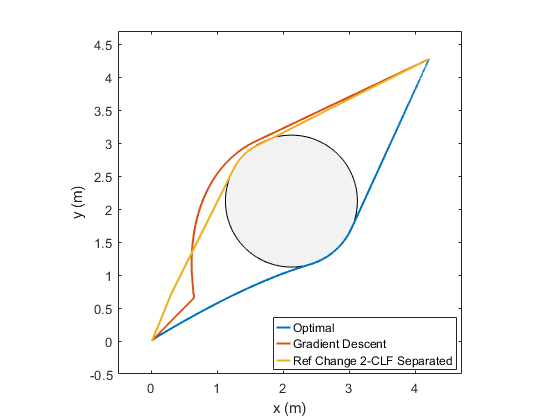
\includegraphics[width=0.99\linewidth]{UCFL.png}
  %\caption{A figure with two sub-figures!}
  \label{fig:UCFL_CostEvol}
  \end{subfigure}
  \begin{subfigure}{0.59\textwidth}
    \centering
    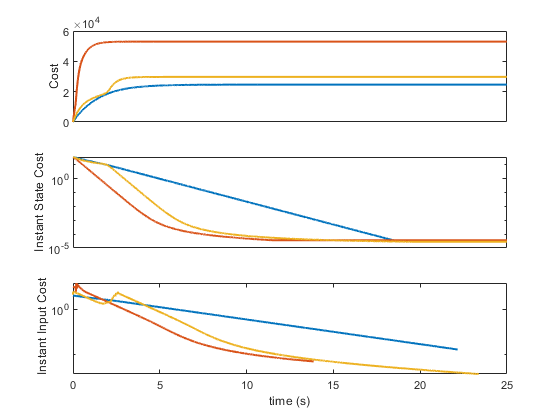
\includegraphics[width=0.95\linewidth]{UCFL_costs.png}
  %\caption{A figure with two sub-figures!}
  \label{fig:UCFL_trajectory}
  \end{subfigure}
  \caption{UCFL~\ref{}}
\label{fig:UCFLTrajectory_and_CostEvol}
\end{figure}



The \glsxtrshort{A-JO} keeps showing the same characteristics in comparison with \glsxtrshort{A-CLF-S} as it was seen in UCCL\ref{ssssec:UCCL}. The \glsxtrshort{A-CLF-S} reveals a relatively similar path to the optimal solution but a faster convergence to \txtref as the \(\gamma\) parameter value (not subject to an optimization) is not suited, which results in higher inputs and penalizing in the total cost. 



  \bgroup
 \rowcolors{1}{}{orange!4}
 \begin{xltabular}{\textwidth}{|l|ccccc|}
   \toprule
   \rowcolor{blue!6}%
   Algorithms   & ComputationalTime  & ReachTime  & InputCost   & StateCost & Cost           \\
   \midrule
    \glsxtrshort{A-JO}~\ref{subsec:Just_Optimized_Algorithm}           & 2.2433 & 13.875  & 49425 & 3756.3 & 53182 \\
    \glsxtrshort{A-CLF-S}~\ref{subsubsec:CLFs_Summed_Algorithm}        & 19.793  & 23.385     & 20190 & 9568.4 & 29758 \\
    \glsxtrshort{A-CLF-I}~\ref{subsubsec:CLFs_Independent_Algorithm}   & ---   & ---      & ---  & ---  & ---  \\
    Optimal (\glsxtrshort{MPC} of 6000 horizon)                        & ---    & 22.16 & 12330  & 12348 & 24678 \\
    \midrule
    \caption{Some UCFL Data}
   \label{tab:Some_UCFL_Data}\\
   \end{xltabular}
 \egroup

 \newpage %so para ajeiutar

\underline{UEV}
\label{UEV} %Unicycle Ellipse Vertical

 \begin{figure}[htbp]
  \begin{subfigure}{0.6\textwidth}
    \centering
    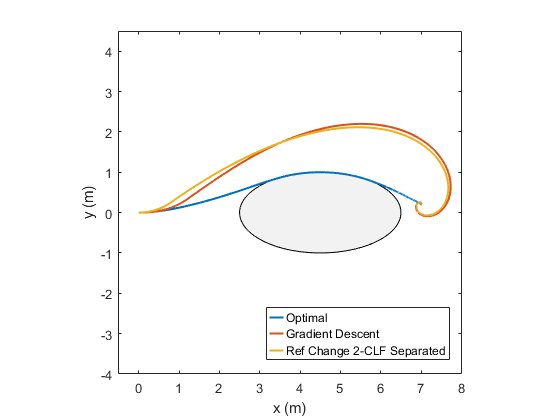
\includegraphics[width=0.99\linewidth]{UEV.png}
  %\caption{A figure with two sub-figures!}
  \label{fig:UEV_CostEvol}
  \end{subfigure}
  \begin{subfigure}{0.59\textwidth}
    \centering
    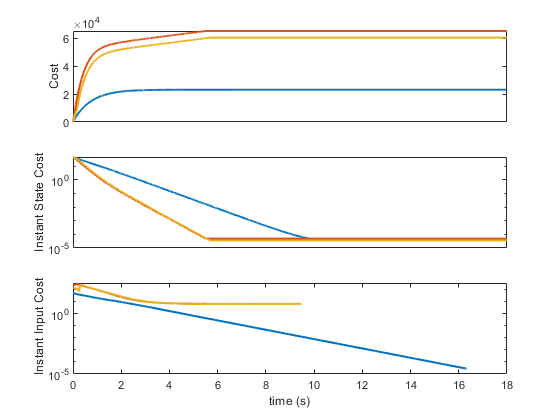
\includegraphics[width=0.95\linewidth]{UEV_costs.png}
  %\caption{A figure with two sub-figures!}
  \label{fig:UEV_trajectory}
  \end{subfigure}
  \caption{UEV~\ref{}}
\label{fig:UEVTrajectory_and_CostEvol}
\end{figure}

Now given an ellipsoidal obstacle, the bigger the axis, making a lower angle with the theoretical vehicle always safe trajectory, relative to the other one the less impactful is \glsxtrshort{A-CLF-S}, not only because of new point demanding a so relevant maneuver but also because of the respective ellipse CBF natural imposure of a more soft avoidance. 


 \bgroup
 \rowcolors{1}{}{orange!4}
 \begin{xltabular}{\textwidth}{|l|ccccc|}
   \toprule
   \rowcolor{blue!6}%
   Algorithms   & ComputationalTime  & ReachTime  & InputCost   & StateCost & Cost           \\
   \midrule
    \glsxtrshort{A-JO}~\ref{subsec:Just_Optimized_Algorithm}           & 3.3449 & 9.185  & 53112 & 4983.7 & 58096 \\
    \glsxtrshort{A-CLF-S}~\ref{subsubsec:CLFs_Summed_Algorithm}        & 9.5229  & 9.485     & 47649 & 5899 & 53547 \\
    \glsxtrshort{A-CLF-I}~\ref{subsubsec:CLFs_Independent_Algorithm}   & ---   & ---      & ---  & ---  & ---  \\
    Optimal (\glsxtrshort{MPC} of 6000 horizon)                        & ---    & 16.315 & 11522  & 11547 & 23069 \\
    \midrule
    \caption{Some UEV Data}
   \label{tab:Some_UEV_Data}\\
   \end{xltabular}
 \egroup


 \glsxtrshort{A-JO} computational time keeps beeing lower than \glsxtrshort{A-CLF-S} but now for an not so worst cost.


  \newpage %so para ajeiutar


\underline{UEH}
\label{UEH} %Unicycle Ellipse Vertical

 \begin{figure}[htbp]
  \begin{subfigure}{0.6\textwidth}
    \centering
    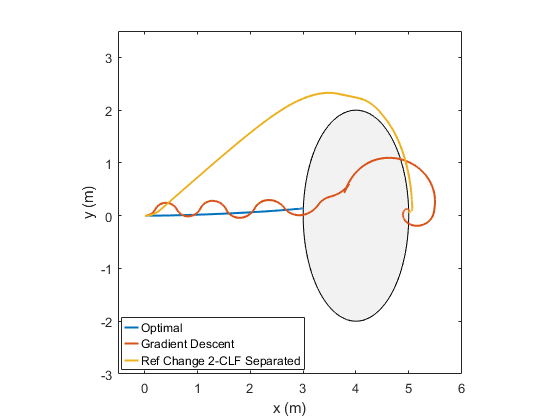
\includegraphics[width=0.99\linewidth]{UEH.png}
  %\caption{A figure with two sub-figures!}
  \label{fig:UEH_CostEvol}
  \end{subfigure}
  \begin{subfigure}{0.59\textwidth}
    \centering
    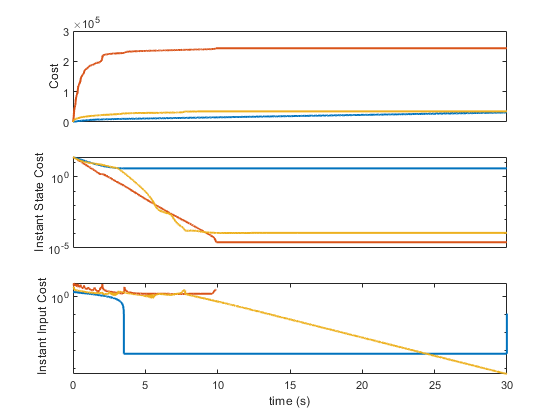
\includegraphics[width=0.95\linewidth]{UEH_costs.png}
  %\caption{A figure with two sub-figures!}
  \label{fig:UEH_trajectory}
  \end{subfigure}
  \caption{UEH~\ref{}}
\label{fig:UEHTrajectory_and_CostEvol}
\end{figure}


If in UEV~\ref{UEV} the \glsxtrshort{A-CLF-S} shows a relative worst performance, in this case its path cost is comparatively considerably better. Beyond that, Aimportant to say that against ellipsoides with its biggest axis near perpendicular to the theoretical vehicle always safe trajectory, or speacially straight surfaces, the best solution given by the \glsxtrshort{CLF-CBF} is to get as much as possible the system close to the obstacle as the \glsxtrshort{CLF-CBF} keeps giving control inputs that lead the system in that instant as close to the \txtref as possible in that exclusive moment, but the \glsxtrshort{A-CLF-S} converging to the contour point is capable to free from it. The \glsxtrshort{MPC} solution presented corresponds to a local minimum, but its path reveals a similar problem to \glsxtrshort{A-JO} due to the finite horizon and its objective function trying to approximate the system as much to \txtref instead of actually optimze its reaching time.


\bgroup
 \rowcolors{1}{}{orange!4}
 \begin{xltabular}{\textwidth}{|l|ccccc|}
   \toprule
   \rowcolor{blue!6}%
   Algorithms   & ComputationalTime  & ReachTime  & InputCost   & StateCost & Cost           \\
   \midrule
    \glsxtrshort{A-JO}~\ref{subsec:Just_Optimized_Algorithm}           & 13.68  & 9.92  & 1.3522e+05 & 3543.4 & 1.3877e+05 \\
    \glsxtrshort{A-CLF-S}~\ref{subsubsec:CLFs_Summed_Algorithm}        & 42.607  & 30     & 21563 & 6332.5 & 27896 \\
    \glsxtrshort{A-CLF-I}~\ref{subsubsec:CLFs_Independent_Algorithm}   & ---   & ---      & ---  & ---  & ---  \\
    Optimal (\glsxtrshort{MPC} of 6000 horizon)                        & ---    & 30 & 3727.1  & 27617 & 31344 \\
    \midrule
    \caption{Some UEH Data}
   \label{tab:Some_UEH_Data}\\
   \end{xltabular}
 \egroup

\begin{tcolorbox}[colback=blue!5!white,colframe=blue!35!white,title=Notes:]
\begin{itemize}
    \item If the constraint is circular, the vehicle is oriented to the \txtref and to the center of the circle the unicycle converges to the obstacle limit.
  \end{itemize}
\end{tcolorbox} 

\newpage %so para ajeitar

\underline{UED}
\label{UED} %Unicycle Ellipse Vertical

 \begin{figure}[htbp]
  \begin{subfigure}{0.6\textwidth}
    \centering
    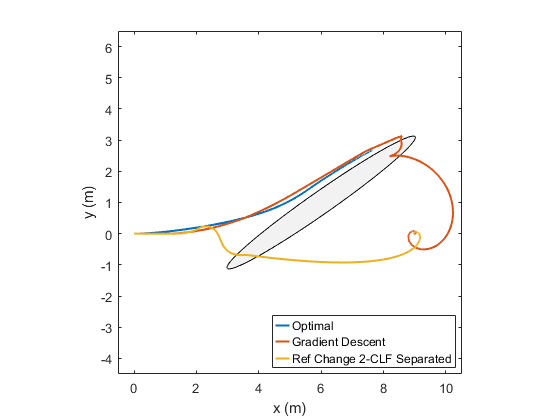
\includegraphics[width=0.99\linewidth]{UED.png}
  %\caption{A figure with two sub-figures!}
  \label{fig:UED_CostEvol}
  \end{subfigure}
  \begin{subfigure}{0.59\textwidth}
    \centering
    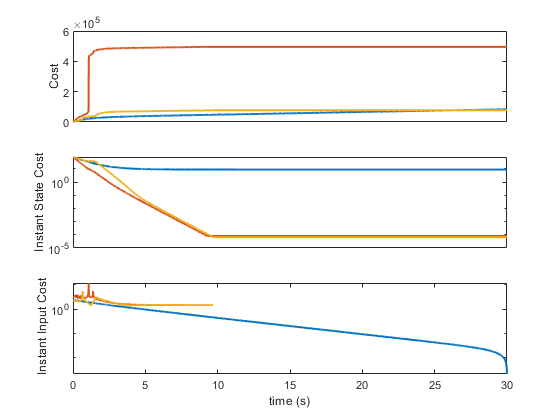
\includegraphics[width=0.95\linewidth]{UED_costs.png}
  %\caption{A figure with two sub-figures!}
  \label{fig:UED_trajectory}
  \end{subfigure}
  \caption{UED~\ref{}}
\label{fig:UEDTrajectory_and_CostEvol}
\end{figure}


As in UEH, although the other techiniques don't keep stuck, the \glsxtrshort{A-CLF-S} keeps showing a better result and the other suffering from the same limitations.


\bgroup
 \rowcolors{1}{}{orange!4}
 \begin{xltabular}{\textwidth}{|l|ccccc|}
   \toprule
   \rowcolor{blue!6}%
   Algorithms   & ComputationalTime  & ReachTime  & InputCost   & StateCost & Cost           \\
   \midrule
    \glsxtrshort{A-JO}~\ref{subsec:Just_Optimized_Algorithm}           & 3.939  & 9.295  & 4.0474e+05 & 8500 & 4.1324e+05 \\
    \glsxtrshort{A-CLF-S}~\ref{subsubsec:CLFs_Summed_Algorithm}        & 53.897 & 9.7     & 43945 & 19422 & 63367 \\
    \glsxtrshort{A-CLF-I}~\ref{subsubsec:CLFs_Independent_Algorithm}   & ---   & ---      & ---  & ---  & ---  \\
    Optimal (\glsxtrshort{MPC} of 6000 horizon)                        & ---    & 30 & 15047  & 69133 & 84180 \\
    \midrule
    \caption{Some UED Data}
   \label{tab:Some_UED_Data}\\
   \end{xltabular}
 \egroup


\subsection{Orbital}
\label{subsec:orbital_experiments}

-mostrar as simulaçoes\\
-explicar os resultados obtidos

















% Most latex users will instead create more and more advanced commands.
% A lot of us have a "commands.tex" that we "\input{commands.text}" at the beginning of all our documents.
% Taking simple examples, I have \newcommand{\CC}{\mathbb{C}} at part of the commands in most of my documents because I use the field of complex number everywhere and \CC is shorter to write than \mathbb{C}. I also have \newenvironment{ctabular}[1]{\begin{center}\begin{tabular}{#1}}{\end{tabular}\end{center}} for whenever I need a centred tabular, which is almost always.

% \makeatletter %Transforma o @ para um caracter normal
% \newcommand{\ntifpkgloaded}{%
%   \@ifpackageloaded% %Não esta ai mas seria mais 3 argumentos {}{}{} o primeiro o package, o segundo e o terceiro if e if not o package tiver sido load respetivamente
% }
% \makeatother %Transforma o @ para um caracter especial outra vez

% \lipsum[1-3]

% \begin{figure}[htbp]
%   \centering
%   \subbottom[One sub-figure\label{fig:leftsubfig}]{%
%     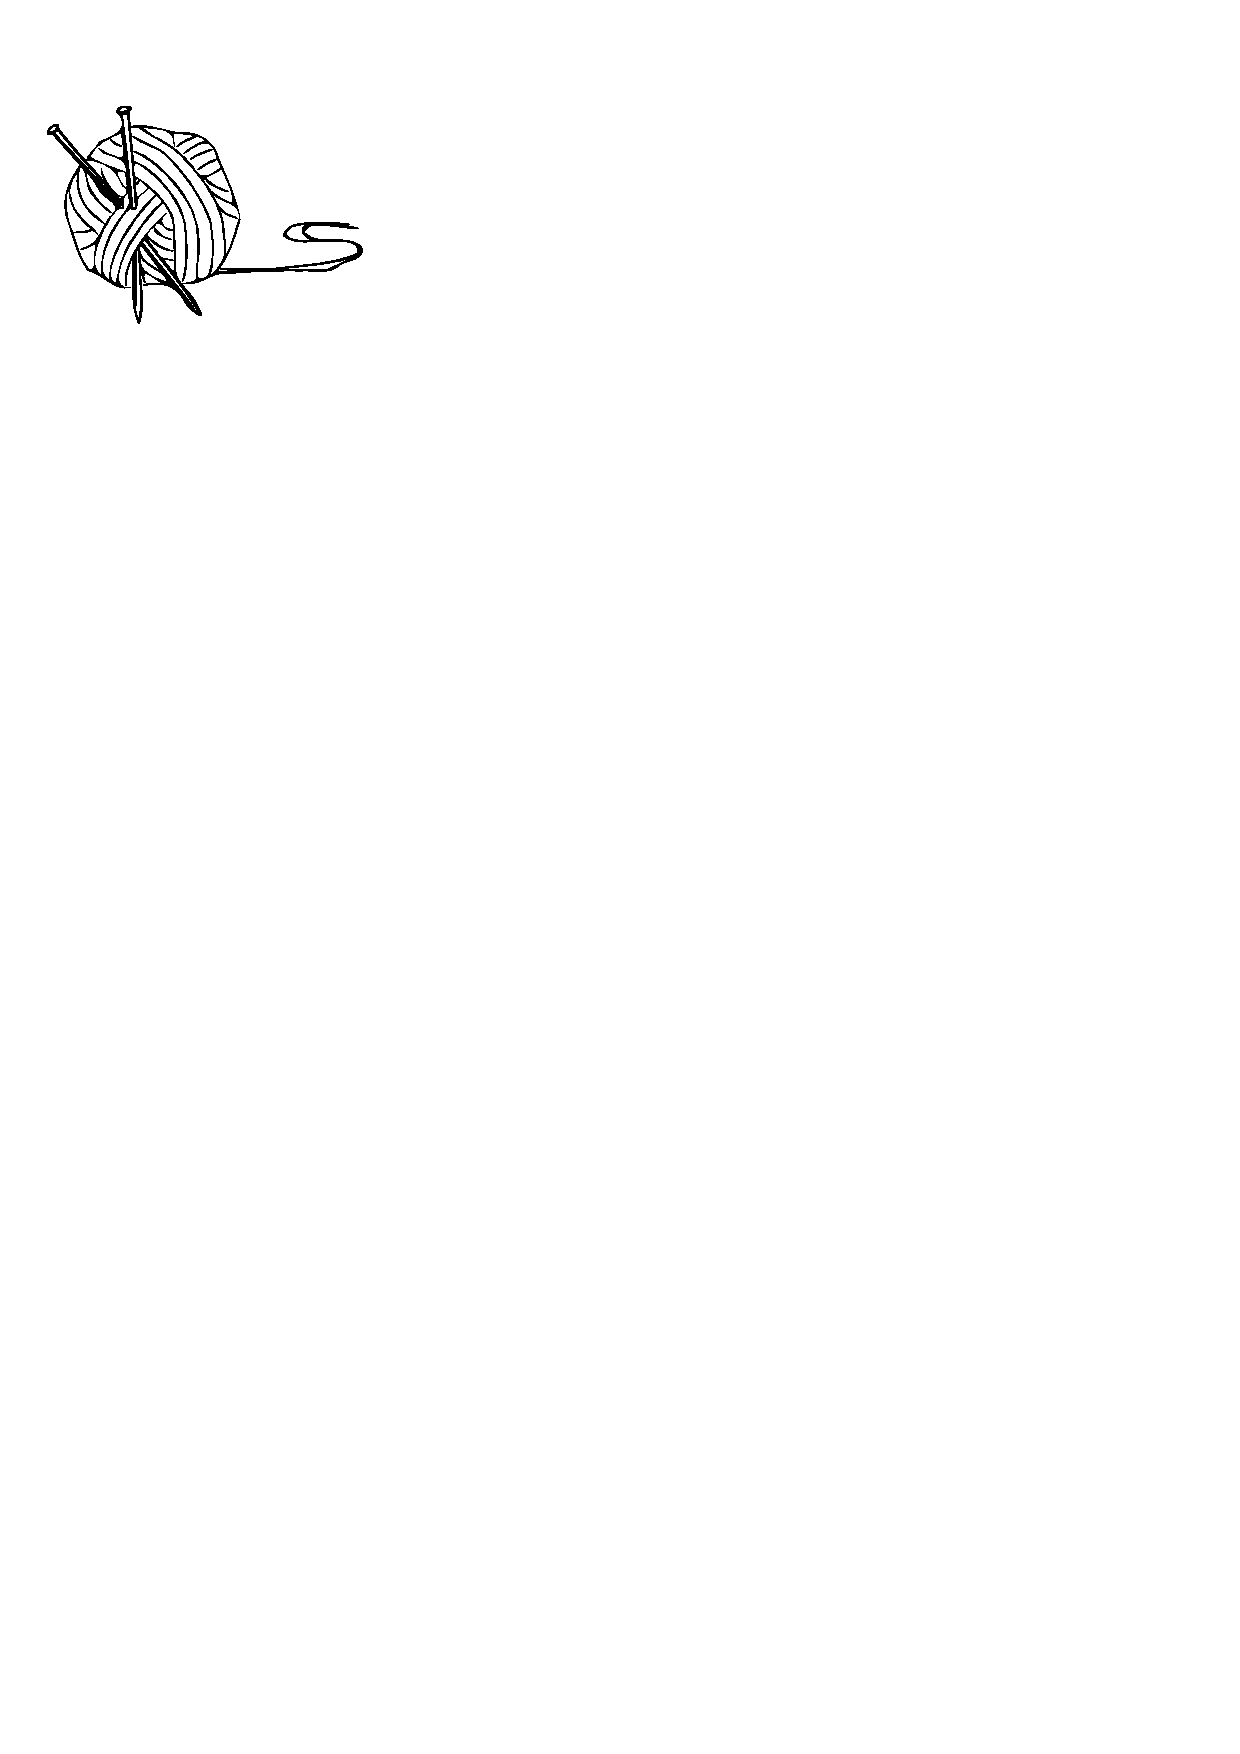
\includegraphics[width=0.5\linewidth]{knitting-vectorial}}%
%   \subbottom[Another sub-figure\label{fig:rightsubfig}]{%
%     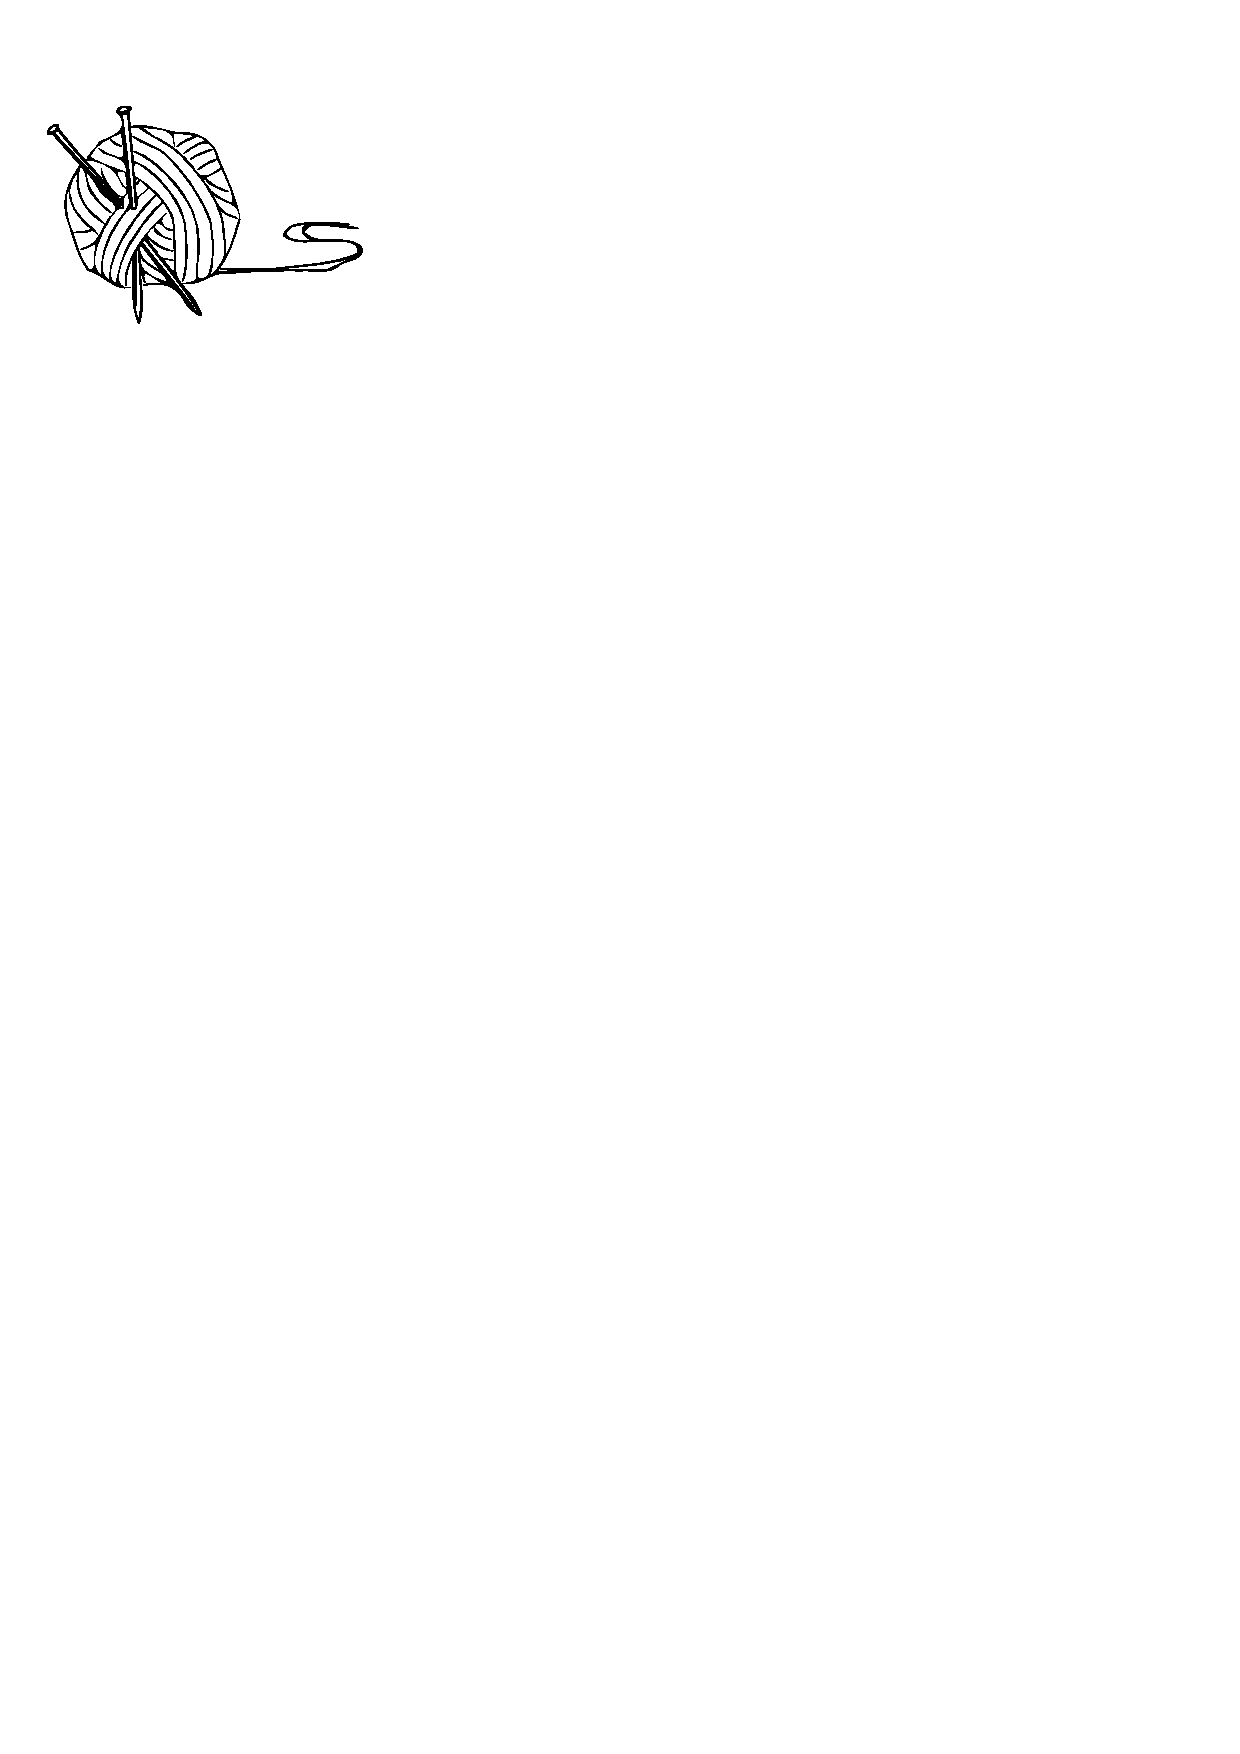
\includegraphics[width=0.5\linewidth]{knitting-vectorial}}%
%   \caption{A figure with two sub-figures!}
%   \label{fig:fig2subfig}
% \end{figure}



%  The Table~\ref{tab:hla:results} illustrates some important concepts associated with table construction:
%  \begin{asparaenum}[i)]
%  \item Do not use vertical lines;
%  \item The caption should be above the table;
%  \item Use the macros \verb!\toprule!, \verb!\midrule! and \verb!\bottomrule! to make the top, inner and bottom horizontal lines, respectively.
%  \end{asparaenum}

%  \bgroup
%  \rowcolors{1}{}{GhostWhite}
%  \begin{xltabular}{\textwidth}{Xccccc}
%    \caption{Test results summary.}
%    \label{tab:hla:results}\\
%    \toprule
%    \rowcolor{Gainsboro}%
%    Test   & Anomalies  & Warnings  & Correct   & Categories            & Missed \\
%    \midrule
%  Connection~\cite{Beckman08}     & 2       & 2          & 1          & \emph{C}              & 1 \\
%  Coordinates'03~\cite{Artho03}   & 1        & 4          & 1          & \emph{2B, 1C}          & 0 \\
%  Local Variable~\cite{Artho03}    & 1        & 2          & 1          & \emph{A}              & 0 \\
%  NASA~\cite{Artho03}              & 1        & 1          & 1          & ---                    & 0 \\
%    \midrule
%    \rowcolor{Gainsboro}%
%  Total                            & 12      & 33        & 10        & 5A, 6B, 10C, 2D       & 2 \\
%    \bottomrule
%    \end{xltabular}
%  \egroup


%  \begin{figure}[htbp]
%    \centering
%    
\includegraphics[height=1in]{snowman-vectorial}
%    
\includegraphics[height=3in]{snowman-vectorial}
%    
\includegraphics[height=6in]{snowman-vectorial}
%    \caption{Vectorial image (PDF)}
%    \label{fig:Figures_Tree_silhouettes-vectorial}
%  \end{figure}

% To combine several figures into a single one… You can then reference the set as Figure~\ref{fig:complete-figure} or the sub-figures separately as~\ref{fig:woolball} and~\ref{fig:cloud}.

% \begin{figure}[htbp]
%   \centering
%     \subbottom[Novelo de lã]{%
%     \label{fig:woolball}
%     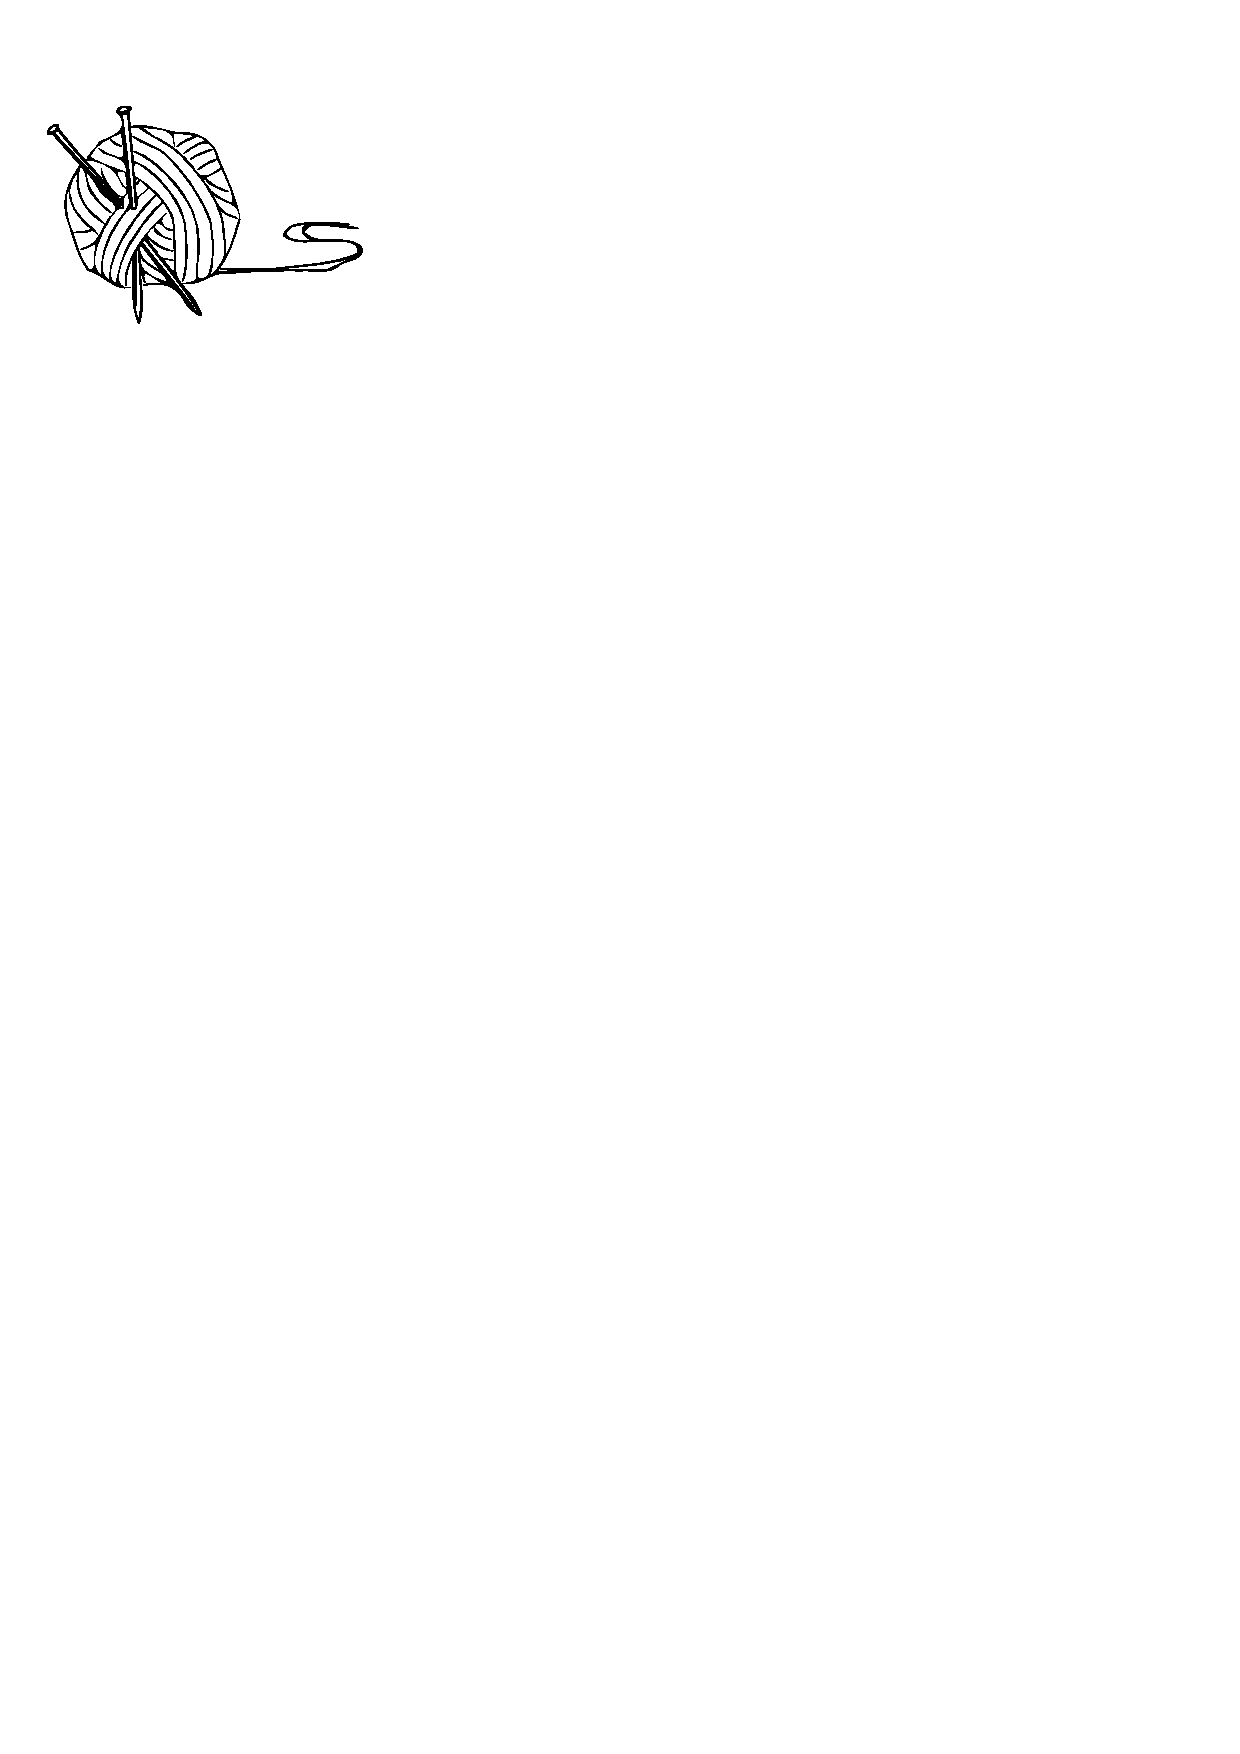
\includegraphics[height=1in]{knitting-vectorial}
%     }
% \qquad\qquad
%     \subbottom[Tempestade com neve]{%
%     \label{fig:cloud}
%     
\includegraphics[height=1in]{snowstorm-vectorial}
%     }
%   \caption{Exemplo de utilização de \emph{subbottom}}
%   \label{fig:complete-figure}
% \end{figure}


% Uncomment the algorithms source below and add the following to file “\verb!5_packages.tex!”
% \begin{verbatim}
%   \usepackage{algorithm2e}
%   \RestyleAlgo{ruled}
% \end{verbatim}
% and uncomment
% \begin{verbatim}
% \ntaddlistof{listofalgorithms}
% \end{verbatim}
% in file “\verb!8_list_og.tex!”.



%NÂO CONSEGUI POR A FUNCIONAR MAS OLHEI POUCO

% \newif\ifntlistingsloaded
% \ntifpkgloaded{listings}{\ntlistingsloadedtrue}{\ntlistingsloadedfalse}
% \newif\ifntmintedloaded
% \ntifpkgloaded{minted}{\ntmintedloadedtrue}{\ntmintedloadedfalse}

% \ifntlistingsloaded
% \section{Test for listings} % (fold)
% \label{sec:test_for_listings}

% Testing the package “listings“…

% \begin{lstlisting}[caption=cap,label=lst:lab,float=htbp]
% if(a==b)
%   puts("YESS!")
% \end{lstlisting}
% \fi

% \ifntmintedloaded
% \section{Test for minted} % (fold)
% \label{sec:test_for_minted}

% Testing the package “minted“…

% \begin{listing}[H]
%   \begin{minted}{C}
%     if(a==b)
%       puts("YESS!")
%   \end{minted}
%   \caption{Example of a listing.}
%   \label{lst:lab}
% \end{listing}
% \fi
